\documentclass[11pt,a4paper]{report}
\usepackage[textwidth=37em,vmargin=30mm]{geometry}
\usepackage{calc,xunicode,amsmath,amssymb,paralist,enumitem,tabu,booktabs,datetime2,xeCJK,xeCJKfntef,listings}
\usepackage{tocloft,fancyhdr,tcolorbox,xcolor,graphicx,eso-pic,xltxtra,xelatexemoji}

\newcommand{\envyear}[0]{2025}
\newcommand{\envdatestr}[0]{2025-08-16}
\newcommand{\envfinaldir}[0]{webdb/2025/20250816/final}

\usepackage[hidelinks]{hyperref}
\hypersetup{
    colorlinks=false,
    pdfpagemode=FullScreen,
    pdftitle={Web Digest - \envdatestr}
}

\setlength{\cftbeforechapskip}{10pt}
\renewcommand{\cftchapfont}{\rmfamily\bfseries\large\raggedright}
\setlength{\cftbeforesecskip}{2pt}
\renewcommand{\cftsecfont}{\sffamily\small\raggedright}

\setdefaultleftmargin{2em}{2em}{1em}{1em}{1em}{1em}

\usepackage{xeCJK,xeCJKfntef}
\xeCJKsetup{PunctStyle=plain,RubberPunctSkip=false,CJKglue=\strut\hskip 0pt plus 0.1em minus 0.05em,CJKecglue=\strut\hskip 0.22em plus 0.2em}
\XeTeXlinebreaklocale "zh"
\XeTeXlinebreakskip = 0pt


\setmainfont{Brygada 1918}
\setromanfont{Brygada 1918}
\setsansfont{IBM Plex Sans}
\setmonofont{JetBrains Mono NL}
\setCJKmainfont{Noto Serif CJK SC}
\setCJKromanfont{Noto Serif CJK SC}
\setCJKsansfont{Noto Sans CJK SC}
\setCJKmonofont{Noto Sans CJK SC}

\setlength{\parindent}{0pt}
\setlength{\parskip}{8pt}
\linespread{1.15}

\lstset{
	basicstyle=\ttfamily\footnotesize,
	numbersep=5pt,
	backgroundcolor=\color{black!5},
	showspaces=false,
	showstringspaces=false,
	showtabs=false,
	tabsize=2,
	captionpos=b,
	breaklines=true,
	breakatwhitespace=true,
	breakautoindent=true,
	linewidth=\textwidth
}






\newcommand{\coverpic}[2]{
    % argv: itemurl, authorname
    Cover photo by #2~~(\href{#1}{#1})
}
\newcommand{\makeheader}[0]{
    \begin{titlepage}
        % \newgeometry{hmargin=15mm,tmargin=21mm,bmargin=12mm}
        \begin{center}
            
            \rmfamily\scshape
            \fontspec{BaskervilleF}
            \fontspec{Old Standard}
            \fontsize{59pt}{70pt}\selectfont
            WEB\hfill DIGEST
            
            \vfill
            % \vskip 30pt
            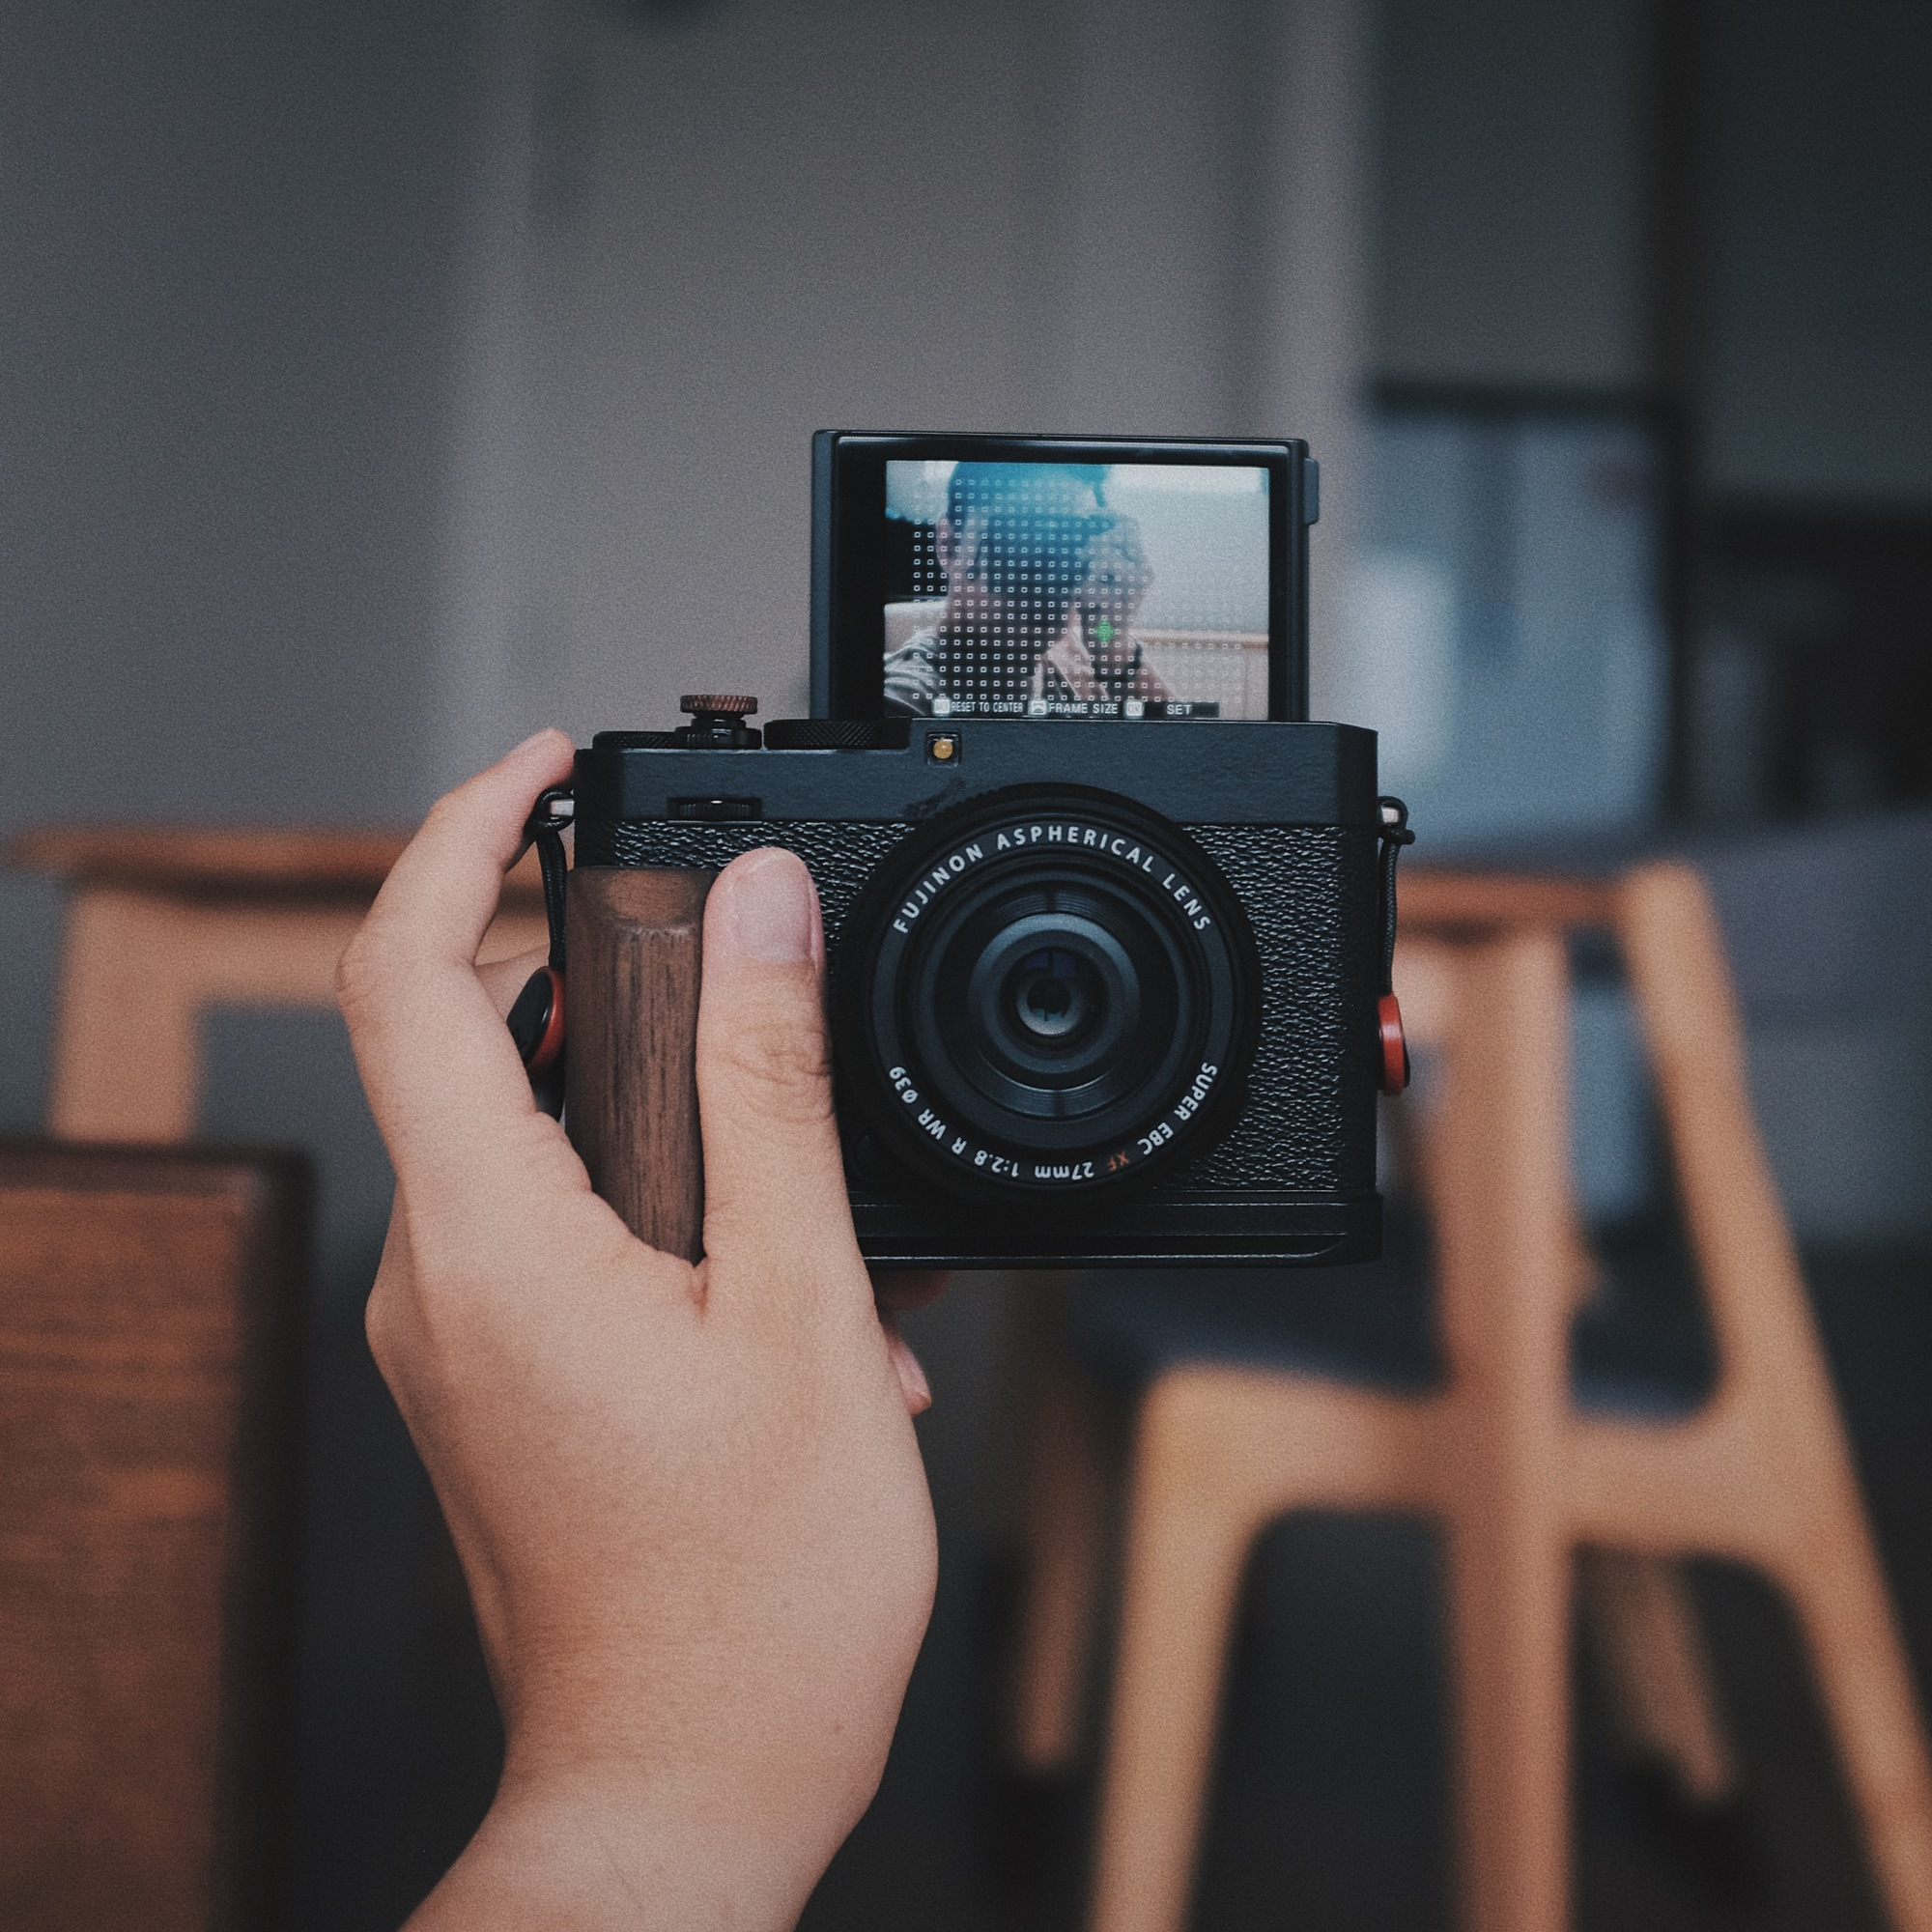
\includegraphics[width=\linewidth]{\envfinaldir/coverpic-prod.jpg}\par
            % \vskip 30pt
            \vfill

            \normalsize\rmfamily\scshape
            \copyright{} The Web Digest Project \hfill\large \envdatestr
        \end{center}
    \end{titlepage}
    % \restoregeometry
}
\newcommand{\simplehref}[1]{%
    \textcolor{blue!80!green}{\href{#1}{#1}}%
}
\renewcommand{\contentsname}{\center\Huge\sffamily\bfseries Contents\par\vskip 20pt}
\newcounter{ipartcounter}
\setcounter{ipartcounter}{0}
\newcommand{\ipart}[1]{
    % \vskip 20pt
    \clearpage
    \stepcounter{ipartcounter}
    \phantomsection
    \addcontentsline{toc}{chapter}{#1}
    % \begin{center}
    %     \Huge
    %     \sffamily\bfseries
    %     #1
    % \end{center}
    % \vskip 20pt plus 7pt
}
\newcounter{ichaptercounter}
\setcounter{ichaptercounter}{0}
\newcommand{\ichapter}[1]{
    % \vskip 20pt
    \clearpage
    \stepcounter{ichaptercounter}
    \phantomsection
    \addcontentsline{toc}{section}{\numberline{\arabic{ichaptercounter}}#1}
    \begin{center}
        \Huge
        \sffamily\bfseries
        #1
    \end{center}
    \vskip 20pt plus 7pt
}
\newcommand{\entrytitlefont}[1]{\subsection*{\raggedright\Large\sffamily\bfseries#1}}
\newcommand{\entryitemGeneric}[2]{
    % argv: title, url
    \parbox{\linewidth}{
        \entrytitlefont{#1}\par\vskip 5pt
        \footnotesize\ttfamily\mdseries
        \simplehref{#2}
    }\vskip 11pt plus 11pt minus 1pt
}
\newcommand{\entryitemGithub}[3]{
    % argv: title, url, desc
    \parbox{\linewidth}{
        \entrytitlefont{#1}\par\vskip 5pt
        \footnotesize\ttfamily\mdseries
        \simplehref{#2}\par\vskip 5pt
        \small\rmfamily\mdseries#3
    }\vskip 11pt plus 11pt minus 1pt
}
\newcommand{\entryitemAp}[3]{
    % argv: title, url, desc
    \parbox{\linewidth}{
        \entrytitlefont{#1}\par\vskip 5pt
        \footnotesize\ttfamily\mdseries
        \simplehref{#2}\par\vskip 5pt
        \small\rmfamily\mdseries#3
    }\vskip 11pt plus 11pt minus 1pt
}
\newcommand{\entryitemHackernews}[3]{
    % argv: title, hnurl, rawurl
    % \parbox{\linewidth}{
    %     \entrytitlefont{#1}\par\vskip 5pt
    %     \footnotesize\ttfamily\mdseries
    %     \simplehref{#3}\par
    %     \textcolor{black!50}{\href{#2}{#2}}
    % }\vskip 11pt plus 11pt minus 1pt
    \begin{minipage}{\linewidth}
            \entrytitlefont{#1}\par\vskip 5pt
            \footnotesize\ttfamily\mdseries
            \simplehref{#3}\par
            \textcolor{black!50}{\href{#2}{#2}}
    \end{minipage}\par\vskip 11pt plus 11pt minus 1pt
}







\begin{document}

\makeheader

\tableofcontents\clearpage




\ipart{Developers}
\ichapter{Hacker News}
\entryitemTwoLinks{Claude Opus 4 and 4.1 can now end a rare subset of conversations}{https://news.ycombinator.com/item?id=44916813}{https://www.anthropic.com/research/end-subset-conversations}

\entryitemTwoLinks{Imagen 4 is now generally available}{https://news.ycombinator.com/item?id=44915187}{https://developers.googleblog.com/en/announcing-imagen-4-fast-and-imagen-4-family-generally-available-in-the-gemini-api/}

\entryitemTwoLinks{Show HN: Edka – Kubernetes clusters on your own Hetzner account}{https://news.ycombinator.com/item?id=44915164}{https://edka.io}

\entryitemTwoLinks{It seems like the AI crawlers learned how to solve the Anubis challenges}{https://news.ycombinator.com/item?id=44914773}{https://social.anoxinon.de/@Codeberg/115033790447125787}

\entryitemTwoLinks{Steam can't escape the fallout from its censorship controversy}{https://news.ycombinator.com/item?id=44914163}{https://www.polygon.com/steam-paypal-issues-censorship-visa-mastercard/}

\entryitemTwoLinks{Occult books digitized and put online by Amsterdam's Ritman Library}{https://news.ycombinator.com/item?id=44914061}{https://www.openculture.com/2025/08/2178-occult-books-now-digitized-put-online.html}

\entryitemTwoLinks{The electric fence stopped working years ago}{https://news.ycombinator.com/item?id=44913663}{https://soonly.com/electric-fences/}

\entryitemTwoLinks{Do Things That Don't Scale (2013)}{https://news.ycombinator.com/item?id=44913359}{https://paulgraham.com/ds.html}

\entryitemTwoLinks{The beauty of a text only webpage}{https://news.ycombinator.com/item?id=44913340}{https://albanbrooke.com/the-beauty-of-a-text-only-webpage/}

\entryitemTwoLinks{ADHD drug treatment and risk of negative events and outcomes}{https://news.ycombinator.com/item?id=44912861}{https://www.bmj.com/content/390/bmj-2024-083658}

\entryitemTwoLinks{The Timmy Trap}{https://news.ycombinator.com/item?id=44912646}{https://jenson.org/timmy/}

\entryitemTwoLinks{White House loyalty rating for companies}{https://news.ycombinator.com/item?id=44912369}{https://www.axios.com/2025/08/15/white-house-rating-big-beautiful-bill}

\entryitemTwoLinks{Is Germany on the brink of banning ad blockers?}{https://news.ycombinator.com/item?id=44912085}{https://blog.mozilla.org/netpolicy/2025/08/14/is-germany-on-the-brink-of-banning-ad-blockers-user-freedom-privacy-and-security-is-at-risk/}

\entryitemTwoLinks{Vaultwarden commit introduces SSO using OpenID Connect}{https://news.ycombinator.com/item?id=44911560}{https://github.com/dani-garcia/vaultwarden/pull/3899}

\entryitemTwoLinks{Open hardware desktop 3D printing is dead?}{https://news.ycombinator.com/item?id=44911423}{https://www.josefprusa.com/articles/open-hardware-in-3d-printing-is-dead/}

\entryitemTwoLinks{Fairness is what the powerful 'can get away with' study shows}{https://news.ycombinator.com/item?id=44911169}{https://phys.org/news/2025-07-fairness-powerful.html}

\entryitemTwoLinks{Court records reveal Sig Sauer knew of pistol risks for years}{https://news.ycombinator.com/item?id=44911069}{https://smokinggun.org/court-records-reveal-sig-sauer-knew-of-pistol-risks-for-years/}

\entryitemTwoLinks{Swiss vs. UK approach to major tranport projects}{https://news.ycombinator.com/item?id=44910393}{https://www.freewheeling.info/blog/swiss-hs2}

\entryitemTwoLinks{UK government states that 'safety' act is about influence over public discourse}{https://news.ycombinator.com/item?id=44910161}{https://bsky.app/profile/tupped.bsky.social/post/3lwgcmswmy222}

\entryitemTwoLinks{Simulating and Visualising the Central Limit Theorem}{https://news.ycombinator.com/item?id=44909133}{https://blog.foletta.net/post/2025-07-14-clt/}\ichapter{Phoronix}
\entryitemGeneric{\hskip 0pt{}GNOME 49 Beta Ships Many Last Minute Features - Including Greater systemd Reliance}{https://www.phoronix.com/news/GNOME-49-Beta}

\entryitemGeneric{\hskip 0pt{}Linux 6.17 Features: Great Intel Graphics Improvements, AMD HFI, Attack Vector Controls + Lenovo Gaming Drivers}{https://www.phoronix.com/review/linux-617-features}

\entryitemGeneric{\hskip 0pt{}Wine 10.13 Released With One Month Worth Of Improvements}{https://www.phoronix.com/news/Wine-10.13-Released}

\entryitemGeneric{\hskip 0pt{}Patches Posted For Raspberry Pi 5 Ethernet With The Upstream Linux Kernel}{https://www.phoronix.com/news/Raspberry-Pi-5-Ethernet-Linux}

\entryitemGeneric{\hskip 0pt{}Ubuntu Developing New "Dangerous" Desktop Images Concept}{https://www.phoronix.com/news/Ubuntu-Dangerous-Desktop}

\entryitemGeneric{\hskip 0pt{}Intel FRED Suffers A Late "Incompatible Change" To The Architecture}{https://www.phoronix.com/news/Intel-FRED-Incompatible-ENDBR64}

\entryitemGeneric{\hskip 0pt{}DM-PCACHE Poised For Linux 6.18 As High Throughput, Low Latency DAX Cache}{https://www.phoronix.com/news/DM-PCACHE-For-Linux-6.18}

\entryitemGeneric{\hskip 0pt{}Generic VFIO Platform Driver To Be Marked As Deprecated For Removal}{https://www.phoronix.com/news/VFIO-Platform-Deprecated}

\entryitemGeneric{\hskip 0pt{}AMD Posts 11th Iteration Of Color Pipeline API For Advanced Color Management On Linux}{https://www.phoronix.com/news/AMD-11th-Color-Pipeline-API}


\ipart{Developers~~~~(zh-Hans)}
\ichapter{Solidot}
\entryitemGeneric{\hskip 0pt{}现阶段的印度越南制造还只是中国加一}{https://www.solidot.org/story?sid=82058}

\entryitemGeneric{\hskip 0pt{}微软高管称语音将成为下一代 Windows 的主要输入方式}{https://www.solidot.org/story?sid=82057}

\entryitemGeneric{\hskip 0pt{}一氧化碳新解毒剂能在数分钟内清理血液}{https://www.solidot.org/story?sid=82056}

\entryitemGeneric{\hskip 0pt{}AI 数据中心推动美国居民电费全面上涨}{https://www.solidot.org/story?sid=82055}

\entryitemGeneric{\hskip 0pt{}广岛和长崎核爆幸存者死于辐射致癌的比例比预期的低}{https://www.solidot.org/story?sid=82054}

\entryitemGeneric{\hskip 0pt{}ReiserFS 在内核的最后残余被清除}{https://www.solidot.org/story?sid=82053}

\entryitemGeneric{\hskip 0pt{}俄罗斯限制 Telegram 和 WhatsApp 的语音呼叫功能}{https://www.solidot.org/story?sid=82052}

\entryitemGeneric{\hskip 0pt{}白宫考虑将对华销售收入上缴模式扩大到其它公司}{https://www.solidot.org/story?sid=82051}

\entryitemGeneric{\hskip 0pt{}DeepSeek 的 R2 模型因华为芯片问题推迟发布}{https://www.solidot.org/story?sid=82050}

\entryitemGeneric{\hskip 0pt{}美国年轻一代更喜欢加速播放视频和音频}{https://www.solidot.org/story?sid=82049}

\entryitemGeneric{\hskip 0pt{}中国推动开源模型令硅谷和华盛顿担忧}{https://www.solidot.org/story?sid=82048}

\entryitemGeneric{\hskip 0pt{}研究认为社交媒体的问题无法得到修正}{https://www.solidot.org/story?sid=82047}

\entryitemGeneric{\hskip 0pt{}挪威指责俄黑客破坏其水坝}{https://www.solidot.org/story?sid=82046}

\entryitemGeneric{\hskip 0pt{}韩国星巴克要求顾客不要将打印机和台式机带到店里}{https://www.solidot.org/story?sid=82045}

\entryitemGeneric{\hskip 0pt{}猫的痴呆症与人类相似}{https://www.solidot.org/story?sid=82044}

\entryitemGeneric{\hskip 0pt{}地震的长尾效应}{https://www.solidot.org/story?sid=82043}

\entryitemGeneric{\hskip 0pt{}美国 在 AI 芯片货物中装定位追踪器}{https://www.solidot.org/story?sid=82042}

\entryitemGeneric{\hskip 0pt{}身份证关联疾病信息}{https://www.solidot.org/story?sid=82041}

\entryitemGeneric{\hskip 0pt{}步行友好的城市增加居民的步行次数}{https://www.solidot.org/story?sid=82040}

\entryitemGeneric{\hskip 0pt{}马斯克威胁苹果,想要提高其 AI 应用 Grok 的排名}{https://www.solidot.org/story?sid=82039}\ichapter{V2EX}
\entryitemGeneric{\hskip 0pt{}[程序员] 一键安装 Debian, Root on ZFS, 支持磁盘加密,支持磁盘压缩,支持远程解锁,有人感兴趣 ZFS On Debian 落地,并一起改进吗?}{https://www.v2ex.com/t/1152782}

\entryitemGeneric{\hskip 0pt{}[分享创造] [原创] 一款功能强大的跨平台 115 网盘第三方桌面客户端(基于开放接口)}{https://www.v2ex.com/t/1152781}

\entryitemGeneric{\hskip 0pt{}[问与答] 大家能登陆汇丰 APP 么?}{https://www.v2ex.com/t/1152780}

\entryitemGeneric{\hskip 0pt{}[程序员] 这种一直访问 /.git/config 的攻击是什么脚本/扫描器吗}{https://www.v2ex.com/t/1152778}

\entryitemGeneric{\hskip 0pt{}[OpenAI] 为什么现在常见的大模型除了美国就是国产的,欧日韩的公司都在干啥?}{https://www.v2ex.com/t/1152777}

\entryitemGeneric{\hskip 0pt{}[分享发现] 写好一篇 blog 之后,可以改一改后多发的高质量的平台整理}{https://www.v2ex.com/t/1152776}

\entryitemGeneric{\hskip 0pt{}[Chrome] 一款开源离线的浏览器主页导航插件}{https://www.v2ex.com/t/1152775}

\entryitemGeneric{\hskip 0pt{}[职场话题] 求求你们不要再因为找不到年薪几十万的工作过来焦虑了🥺}{https://www.v2ex.com/t/1152774}

\entryitemGeneric{\hskip 0pt{}[程序员] 请教 AIstudio 上的 Gemini 2.5 pro 回复几轮后就不思考直接回复,隔壁站帖子提示词试了还是没太大作用。}{https://www.v2ex.com/t/1152773}

\entryitemGeneric{\hskip 0pt{}[宽带症候群] 从应用角度来说, IPv6 是否可以说,彻底失败啦?}{https://www.v2ex.com/t/1152772}

\entryitemGeneric{\hskip 0pt{}[分享发现] 🎮 「Grow a Garden」精准计算器发布:全变种/突变/好友加成一站式计算}{https://www.v2ex.com/t/1152771}

\entryitemGeneric{\hskip 0pt{}[Solana] 刚才突然想做一个国内稳定币换 v 币的交互网站}{https://www.v2ex.com/t/1152770}

\entryitemGeneric{\hskip 0pt{}[问与答] 关于 oauth2 登录,前后端分离的项目,请教我这样的实现是符合安全规范和最佳实践的吗?}{https://www.v2ex.com/t/1152768}

\entryitemGeneric{\hskip 0pt{}[远程工作] 招聘,公司岗位内推,产品经理(链上数据),后端工程师(Web3 方向), QA 工程师(侧重测试开发)}{https://www.v2ex.com/t/1152767}

\entryitemGeneric{\hskip 0pt{}[生活] 小区楼下宠物店一直有狗叫怎么办最有效?对方表示整改但是随机复现}{https://www.v2ex.com/t/1152766}

\entryitemGeneric{\hskip 0pt{}[Solana] V2EX 是底了嘛?我先冲了}{https://www.v2ex.com/t/1152765}

\entryitemGeneric{\hskip 0pt{}[宽带症候群] 上海联通最近高峰期 technology 有点慢啊}{https://www.v2ex.com/t/1152764}

\entryitemGeneric{\hskip 0pt{}[问与答] rime for macos 个人词库养成 办法讨论}{https://www.v2ex.com/t/1152763}

\entryitemGeneric{\hskip 0pt{}[Solana] \$V2EX 打赏已经开启了第一波赋能!}{https://www.v2ex.com/t/1152762}

\entryitemGeneric{\hskip 0pt{}[酷工作] [广州-三七互娱-社招内推-技术最新汇总]AI 应用开发工程师、AIGC 算法工程师、高级/资深测试工程师、高级 AI 产品经理、 Java 全栈开发工程师(2 个 hc)、基础运维工程师、运维开发工程师、golang 后端开发、数据分析师}{https://www.v2ex.com/t/1152761}

\entryitemGeneric{\hskip 0pt{}[Linux] 有没有 MacBook Air 品质的 Linux 笔记本?}{https://www.v2ex.com/t/1152760}

\entryitemGeneric{\hskip 0pt{}[问与答] 欧美不应该版权更严格么,为啥留学生都会去 千帆影视 厂长资源 爱一帆这种看电视}{https://www.v2ex.com/t/1152759}

\entryitemGeneric{\hskip 0pt{}[Solana] \$V2EX 又到了一个关键节点, 大家都抄底了吗?}{https://www.v2ex.com/t/1152756}

\entryitemGeneric{\hskip 0pt{}[程序员] 现在搞一个产品官网, 要支持 i18n, 方便 seo 等, 用什么技术栈比较好}{https://www.v2ex.com/t/1152755}

\entryitemGeneric{\hskip 0pt{}[程序员] Windsurf 被收购后, 第一波牛逼功能来了: 集成 Deepwiki 🔥🔥🔥}{https://www.v2ex.com/t/1152754}

\entryitemGeneric{\hskip 0pt{}[问与答] 求推荐一个物美价廉的图床服务}{https://www.v2ex.com/t/1152753}

\entryitemGeneric{\hskip 0pt{}[问与答] Jetbrains 教育许可证过期了,如何删除?}{https://www.v2ex.com/t/1152750}

\entryitemGeneric{\hskip 0pt{}[问与答] 请问一下现在境外证券开户还有哪些能开,推荐用什么?谢谢大佬。}{https://www.v2ex.com/t/1152748}

\entryitemGeneric{\hskip 0pt{}[Ripple] 谁在 okx 持有 xrp 吗?}{https://www.v2ex.com/t/1152747}

\entryitemGeneric{\hskip 0pt{}[宽带症候群] [求助] 哪家国内云的 ipv6 国内节点连接外国带宽线路好?}{https://www.v2ex.com/t/1152746}

\entryitemGeneric{\hskip 0pt{}[macOS] 救命, mac 上的 outlook 的邮件丢了,十万火急}{https://www.v2ex.com/t/1152745}

\entryitemGeneric{\hskip 0pt{}[全球工单系统] V2er 最近不好使了,求开发者更新下}{https://www.v2ex.com/t/1152744}

\entryitemGeneric{\hskip 0pt{}[Solana] 请教一个关于 priority fee 的问题}{https://www.v2ex.com/t/1152743}

\entryitemGeneric{\hskip 0pt{}[问与答] 脱产学英语是个好的选择吗?}{https://www.v2ex.com/t/1152742}

\entryitemGeneric{\hskip 0pt{}[MacBook Air] M4 Macbook + Win 双系统 kvm 解决方案?}{https://www.v2ex.com/t/1152741}

\entryitemGeneric{\hskip 0pt{}[问与答] 海康威视 rtsp 源截取的视频帧大面积灰色的问题}{https://www.v2ex.com/t/1152740}

\entryitemGeneric{\hskip 0pt{}[程序员] 前端页面支持多语言 I8N 改造当前项目好费劲}{https://www.v2ex.com/t/1152739}

\entryitemGeneric{\hskip 0pt{}[问与答] 为什么机顶盒接路由器上就不行了呢}{https://www.v2ex.com/t/1152738}

\entryitemGeneric{\hskip 0pt{}[问与答] 堡垒机使用痛点调查}{https://www.v2ex.com/t/1152737}

\entryitemGeneric{\hskip 0pt{}[分享发现] 说一个事让大家笑笑}{https://www.v2ex.com/t/1152736}

\entryitemGeneric{\hskip 0pt{}[Solana] 20250815 - 打赏界面更新,现在已经支持发送 \$V2EX 打赏}{https://www.v2ex.com/t/1152735}

\entryitemGeneric{\hskip 0pt{}[程序员] 使用 wireguard 转发跳板机上的 socks 代理,闲置 10~12 秒的 TCP 连接总是会自动关闭,怎么排查是什么原因?(客户端、服务器均在美国)}{https://www.v2ex.com/t/1152733}

\entryitemGeneric{\hskip 0pt{}[分享创造] [分享] 一款基于 Web 的 MCP 客户端可以快速访问基于 SSE 和 Streamable HTTP 类型的各种 MCP 服务器,方便快捷,即用即走。}{https://www.v2ex.com/t/1152732}

\entryitemGeneric{\hskip 0pt{}[问与答] 今天想搬出去租房住,感觉和父母真的很不同频,但是他们不理解,大吵大闹,我该怎么办?}{https://www.v2ex.com/t/1152731}

\entryitemGeneric{\hskip 0pt{}[问与答] 请教关于多用户编辑 PDF 时遇到的问题}{https://www.v2ex.com/t/1152729}

\entryitemGeneric{\hskip 0pt{}[路由器] 请推荐作软路由的 mini PC}{https://www.v2ex.com/t/1152728}

\entryitemGeneric{\hskip 0pt{}[加密货币] 请问现在注册 SafePal 还有什么新人活动可以薅吗?}{https://www.v2ex.com/t/1152727}

\entryitemGeneric{\hskip 0pt{}[问与答] 求一个简单的任务分配管理工具}{https://www.v2ex.com/t/1152726}

\entryitemGeneric{\hskip 0pt{}[投资] 当越来越多人开始讨论股票时,总感觉不太妙}{https://www.v2ex.com/t/1152725}

\entryitemGeneric{\hskip 0pt{}[推广] 周五加班到 8 点?不存在的。躲进会议室,语音 7× 速写代码, 6 点前下班}{https://www.v2ex.com/t/1152724}


\ipart{Generic News}







\clearpage
\leavevmode\vfill
\footnotesize

Copyright \copyright{} 2023-2025 Neruthes and other contributors.

This document is published with CC BY-NC-ND 4.0 license.

The entries listed in this newsletter may be copyrighted by their respective creators.

This newsletter is generated by the Web Digest project.

The newsletters are also delivered via Telegram channel \CJKunderline{\href{https://t.me/webdigestchannel}{https://t.me/webdigestchannel}}.\\
RSS feed is available at \CJKunderline{\href{https://webdigest.pages.dev/rss.xml}{https://webdigest.pages.dev/rss.xml}}.

This newsletter is available in PDF at
\CJKunderline{\href{https://webdigest.pages.dev/}{https://webdigest.pages.dev/}}.

The source code being used to generate this newsletter is available at\\
\CJKunderline{\href{https://github.com/neruthes/webdigest}{https://github.com/neruthes/webdigest}}.

This newsletter is also available in
\CJKunderline{\href{http://webdigest.pages.dev/readhtml/\envyear/WebDigest-20250816.html}{HTML}} and
\CJKunderline{\href{https://github.com/neruthes/webdigest/blob/master/markdown/\envyear/WebDigest-20250816.md}{Markdown}}.


\coverpic{https://unsplash.com/photos/vendor-at-a-market-selling-fresh-colorful-produce-bUBrF-5kvPw}{thinh nguyen}


\end{document}
